\section{Discussion and Analysis}
\label{sec:discussion}
\shrink
In this section, we provide further analyses by investigating the learning pace in \cws and \fwl, the bias-variance trade-off in \fwl, the sensitivity of \fwl to the quality of weak labels, and how modulating the learning rate in \fwl can be different from the weighted sampling of training samples.

\subsection{Faster Learning Pace in \cws}
\label{sec:learning_pace}
\begin{figure}[!t]%
    \centering
    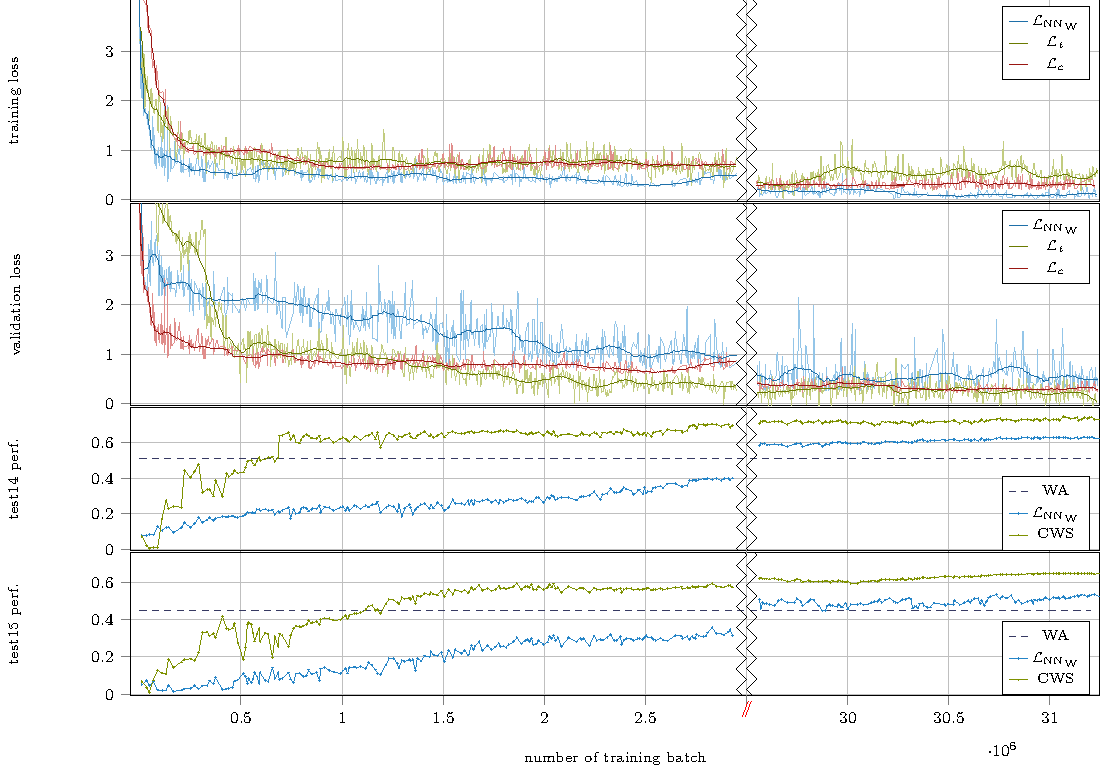
\includegraphics[width=0.95\textwidth]{03-part-02/chapter-05/figs_and_tables/plot_loss_cws.pdf}
    \caption{Loss of the \tnet ($\mathcal{L}_t$) and the \cnet ($\mathcal{L}_c$) compared to the loss of $\text{NN}_{\text{W}}$ ($\mathcal{L}_{\text{NN}_{\text{W}}}$) on training/validation set and performance of \cws, $\text{NN}_{\text{W}}$, and \wa on test sets with respect to different amount of training data on sentiment classification.}
    \label{fig:plot_loss_cws}
\end{figure}
In \cws, controlling the contribution of the weak labels to updating the parameters of the model not only improves the performance, but also provides the network with more solid signals, which speeds up the learning process. 

Figure~\ref{fig:plot_loss_cws} illustrates the training/validation loss for both networks compared to the loss of training the \tnet with weak supervision, along with their performance on test sets, with respect to different amounts of training data for the sentiment classification task we observed a similar pattern for the document ranking task.

As shown, in training, the loss of the \tnet in our model, i.e., $\mathcal{L}_t$ is higher than the loss of the network that is trained only on weakly supervised data, i.e., $\mathcal{L}_{\text{NN}_{\text{W}}}$. 
%
However, since these losses are calculated with respect to the weak labels (not true labels), having very low training loss can be an indication of overfitting to the imperfection of weak labels. 
%
In other words, regardless of the general problem of lack of generalization due to overfitting, in the setup of learning from weak labels, predicting labels that are similar to train labels (very low training loss) is not necessarily a desirable incident. 

In the validation set, however, $\mathcal{L}_t$ decreases faster than $\mathcal{L}_{\text{NN}_{\text{W}}}$, which supports the fact that $\mathcal{L}_{\text{NN}_{\text{W}}}$ overfits to the imperfection of weak labels, while our setup helps the \tnet to escape from this imperfection and do an excellent job on the validation set.
%
In terms of the performance, compared to $\text{NN}_{\text{W}}$, the performance of CWS on both test sets increases very quickly and CWS can pass the performance of the \wa by seeing much fewer instances annotated by the \wa.
\subsection{A Good Teacher is Better than Many Observations} 

We look at the rate of learning for the \std in \fwl as the amount of training data is varied. This experiment is related to the connection of \fwl with Vapnik's \emph{learning using privileged information} (LUPI)~\citep{vapnik2009new, vapnik2015learning}, thus,  we first  highlight this connection.

\subsubsection{Connection with Vapnik's LUPI}
\label{sec:LUPI}
\fwl makes use of information from a small set of correctly labeled data to improve the performance of a semi-supervised learning algorithm. The main idea behind LUPI comes from the fact that humans learn much faster than machines. This can be due to the role that an \emph{Intelligent Teacher} plays in human learning. In this framework, the training data is a collection of triplets
\begin{equation}
    \{(x_1, y_1, x_1^*),\ldots,(x_n,y_n,x_n^*)\}\mathtt{\sim}P^n(x,y,x^*),
\end{equation}
where each ${(x_i,y_i)}$ is a pair of feature-label and $x_i^*$ is the additional information provided by an intelligent teacher to ease the learning process for the \std. Additional information for each ${(x_i,y_i)}$ is available only during training time and the learning machine must only rely on $x_i$ at test time. The theory of LUPI studies how to leverage such a teaching signal $x_i^*$ to outperform learning algorithms utilizing only the normal features $x_i$. For example, MRI brain images can be augmented with high-level medical or even psychological descriptions of Alzheimer's disease to build a classifier that predicts the probability of Alzheimer's disease from an MRI image at test time.
It is known from statistical learning theory~\citep{Vapnik1998} that the following bound for test error is satisfied with probability $1-\delta$:
\begin{equation}
\label{eq:LUPI_error_bound}
    R(f) \leq R_n(f) + O\left(\left(\frac{|\mathcal{F}|_{VC}-\log \sigma}{n}\right)^\alpha\right),
\end{equation}
where $R_n(f)$ denotes the training error over $n$ samples, $|\mathcal{F}|_{VC}$ is the VC dimension of the space of functions from which $f$ is chosen, and $\alpha \in [0.5,1]$. When the classes are not $separable$, $\alpha = 0.5$ i.e., the machine learns at a slow rate of $O(n^{-1/2})$. For easier problems where classes are $separable$, $\alpha=1$ resulting in a learning rate of $O(n^{-1})$.  The difference between these two cases is severe. The same error bound achieved for a separable problem with 10 thousand data points is only obtainable for a non-separable problem when 100 million data points are provided. This is prohibitive even when obtaining large datasets is not so costly. 

The theory of LUPI shows that an intelligent teacher can reduce $\alpha$ resulting in a faster learning process for the student. In this chapter, we have proposed a \emph{teacher}-\emph{student} framework for semi-supervised learning. Similar to LUPI, in \fwl a student is supposed to solve the main prediction task while an intelligent teacher provides additional information to improve its learning. In addition, we first train the \std network so that it obtains initial knowledge of weakly labeled data and learns a good data representation. Then the \tch is trained on truly labeled data enjoying the representation learned by the \std. This extends LUPI in a way that the \tch provides privileged information that is most useful for the current state of \std's knowledge. \fwl also extends LUPI by introducing several teachers each of which is specialized to correct the \std's knowledge related to a specific region of the data space.

% Figure~\ref{fig:learning_rate}(a) provides evidence for the assumption that privileged information in our task can accelerate the learning process of the \std. It shows how the privileged information from an intelligent teacher affects the exponent $\alpha$ of the error bound in Equation~\ref{eq:LUPI_error_bound}. Figure~\ref{fig:learning_rate}(b) shows the test error for various number of samples $|\mathcal{D}_s|$ with true label. As expected, In both extremes where $|\mathcal{D}_s|$ is too small or too large, the performance of our model becomes close to the models without a teacher. The reason is that \std has enough strong samples to learn a good model of true function. In more realistic cases where $|\mathcal{D}_s|\ll|\mathcal{D}_w|$ but $|\mathcal{D}_s|$ is still large enough to be informative about $|\mathcal{D}_w|$, our model gives a lower test error than models without the intelligent teacher.

The theory of LUPI was first developed and proved for support vector machines by Vapnik as a method for knowledge transfer. Hinton introduced~\emph{dark knowledge} as a spiritually close idea in the context of neural networks~\citep{Hinton:2006}. He proposed to use a large network or an ensemble of networks for training and a smaller network at test time. It turned out that compressing knowledge of a large system into a smaller system can improve the generalization ability. It was shown 
%in~\citep{lopez2015unifying} 
in~\citep{lopez:2015} that dark knowledge and LUPI can be unified under a single umbrella, called \emph{generalized distillation}. The core idea of these models is \emph{machines-teaching-machines}. As the name suggests, a machine is learning the knowledge embedded in another machine. In our case, the \std is correcting its knowledge by receiving privileged information about label uncertainty from the \tch. 

\fwl extends the core idea of LUPI in the following directions:
\begin{itemize}[leftmargin=*]%
%save some space
\setlength{\topsep}{0.1pt}
\setlength{\partopsep}{0.1pt}
\setlength{\itemsep}{0.1pt}
\setlength{\parskip}{0.1pt}
\setlength{\parsep}{0.1pt}
    \item Trainable teacher: It is often assumed that the teacher in LUPI framework has some additional true information. We show that when this extra information is not available, one can still use the LUPI setup and define an implicit teacher whose knowledge is learned from the true data. In this approach, the performance of the final \std-\tch system depends on a clever answer to the following question: which information should be considered as the privileged knowledge of \tch.
  \item Bayesian teacher: The proposed teacher is Bayesian. It provides posterior uncertainty of the label of each sample.
  \item Mutual representation: We introduced module $\psi(\cdot)$ that learns a mutual embedding (representation) for both \std and teacher. This is in particular interesting because it defines a two-way channel between teacher and \std. 
  \item Multiple teachers: We proposed a scalable method to introduce several teachers such that each teacher is specialized in a particular region of the data space.
\end{itemize}

\begin{figure}[!t]%
    \centering
    \begin{subfigure}[t]{0.7\textwidth}
        \centering
        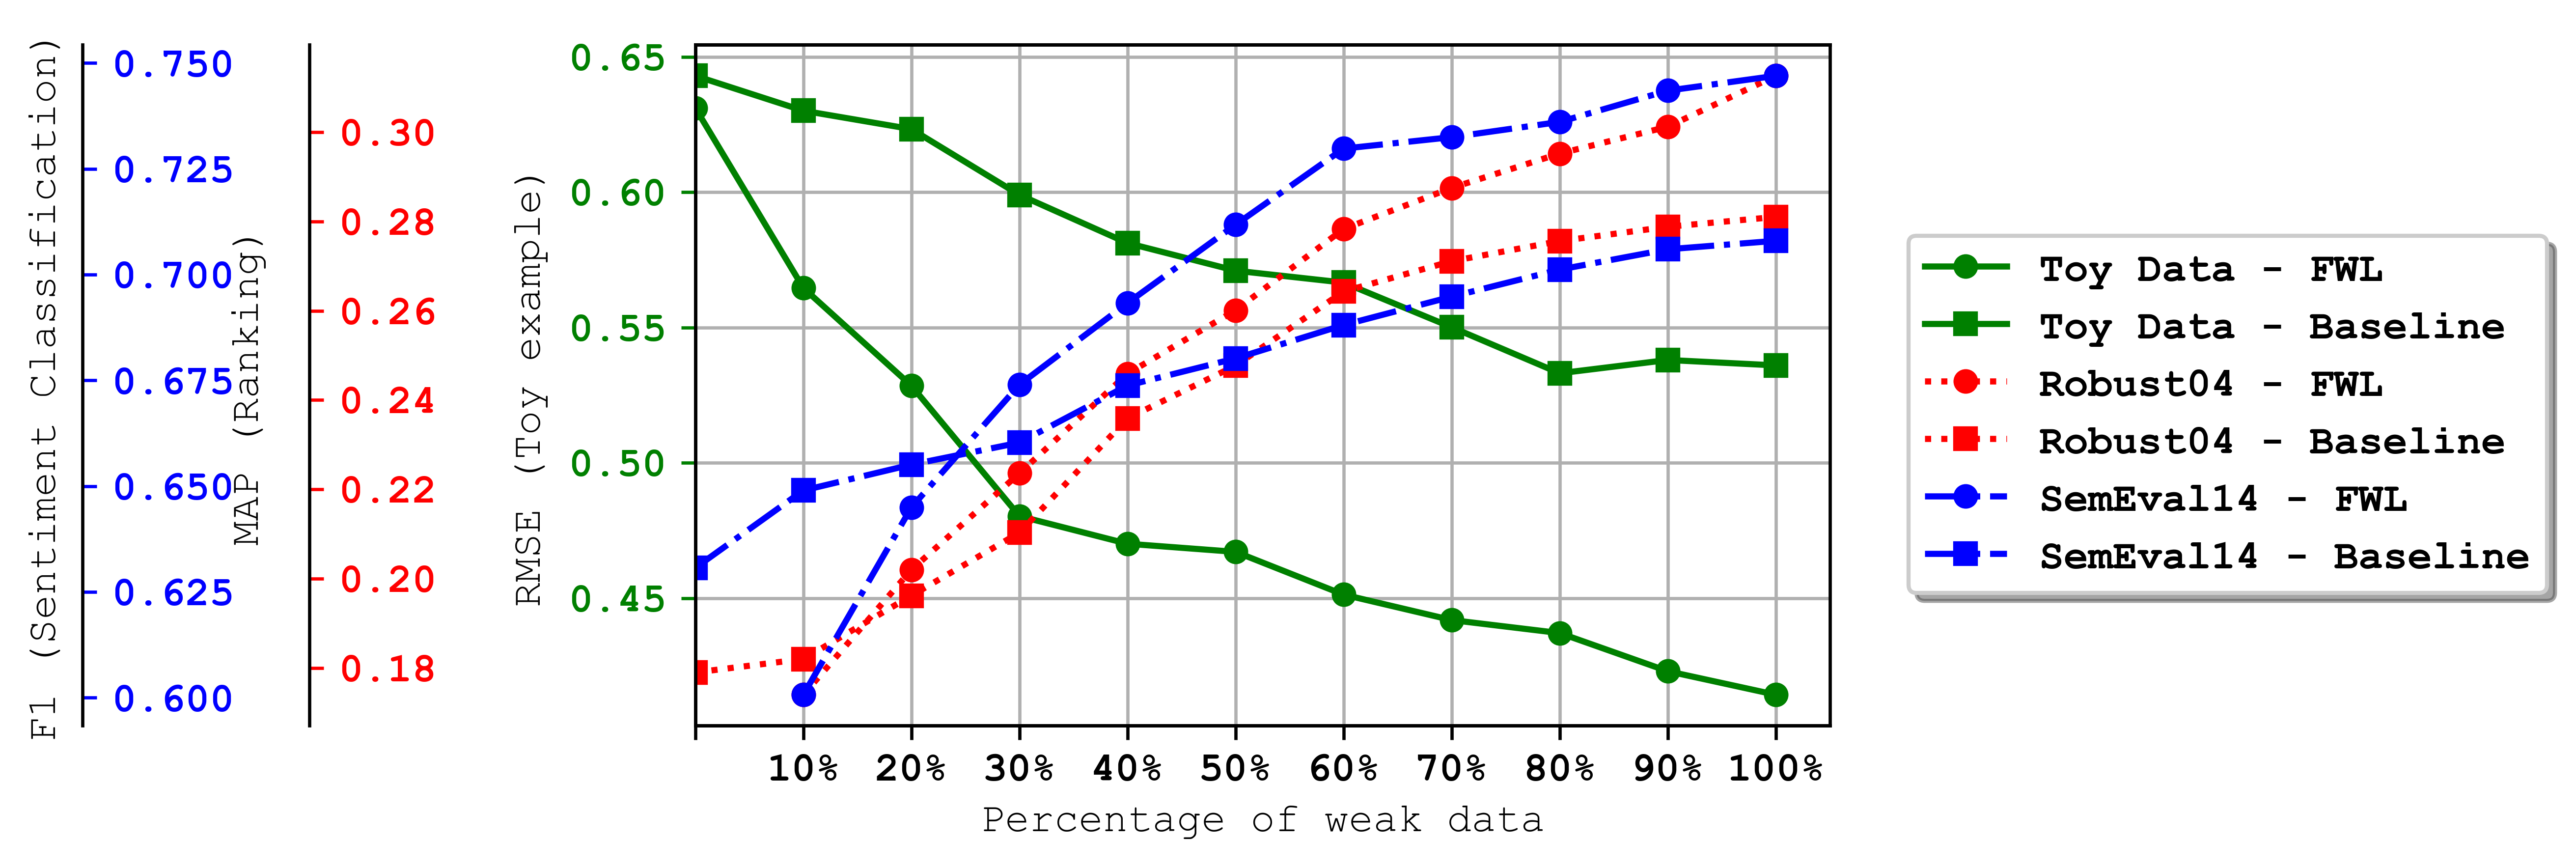
\includegraphics[width=\textwidth]{03-part-02/chapter-05/figs_and_tables/fig_data_w.png}
        \caption{\label{fig:plot_dw}\footnotesize{Models trained on different amount of weak data.}}
    \end{subfigure}%
    \hfill
    \begin{subfigure}[t]{0.7\textwidth}
        \centering
        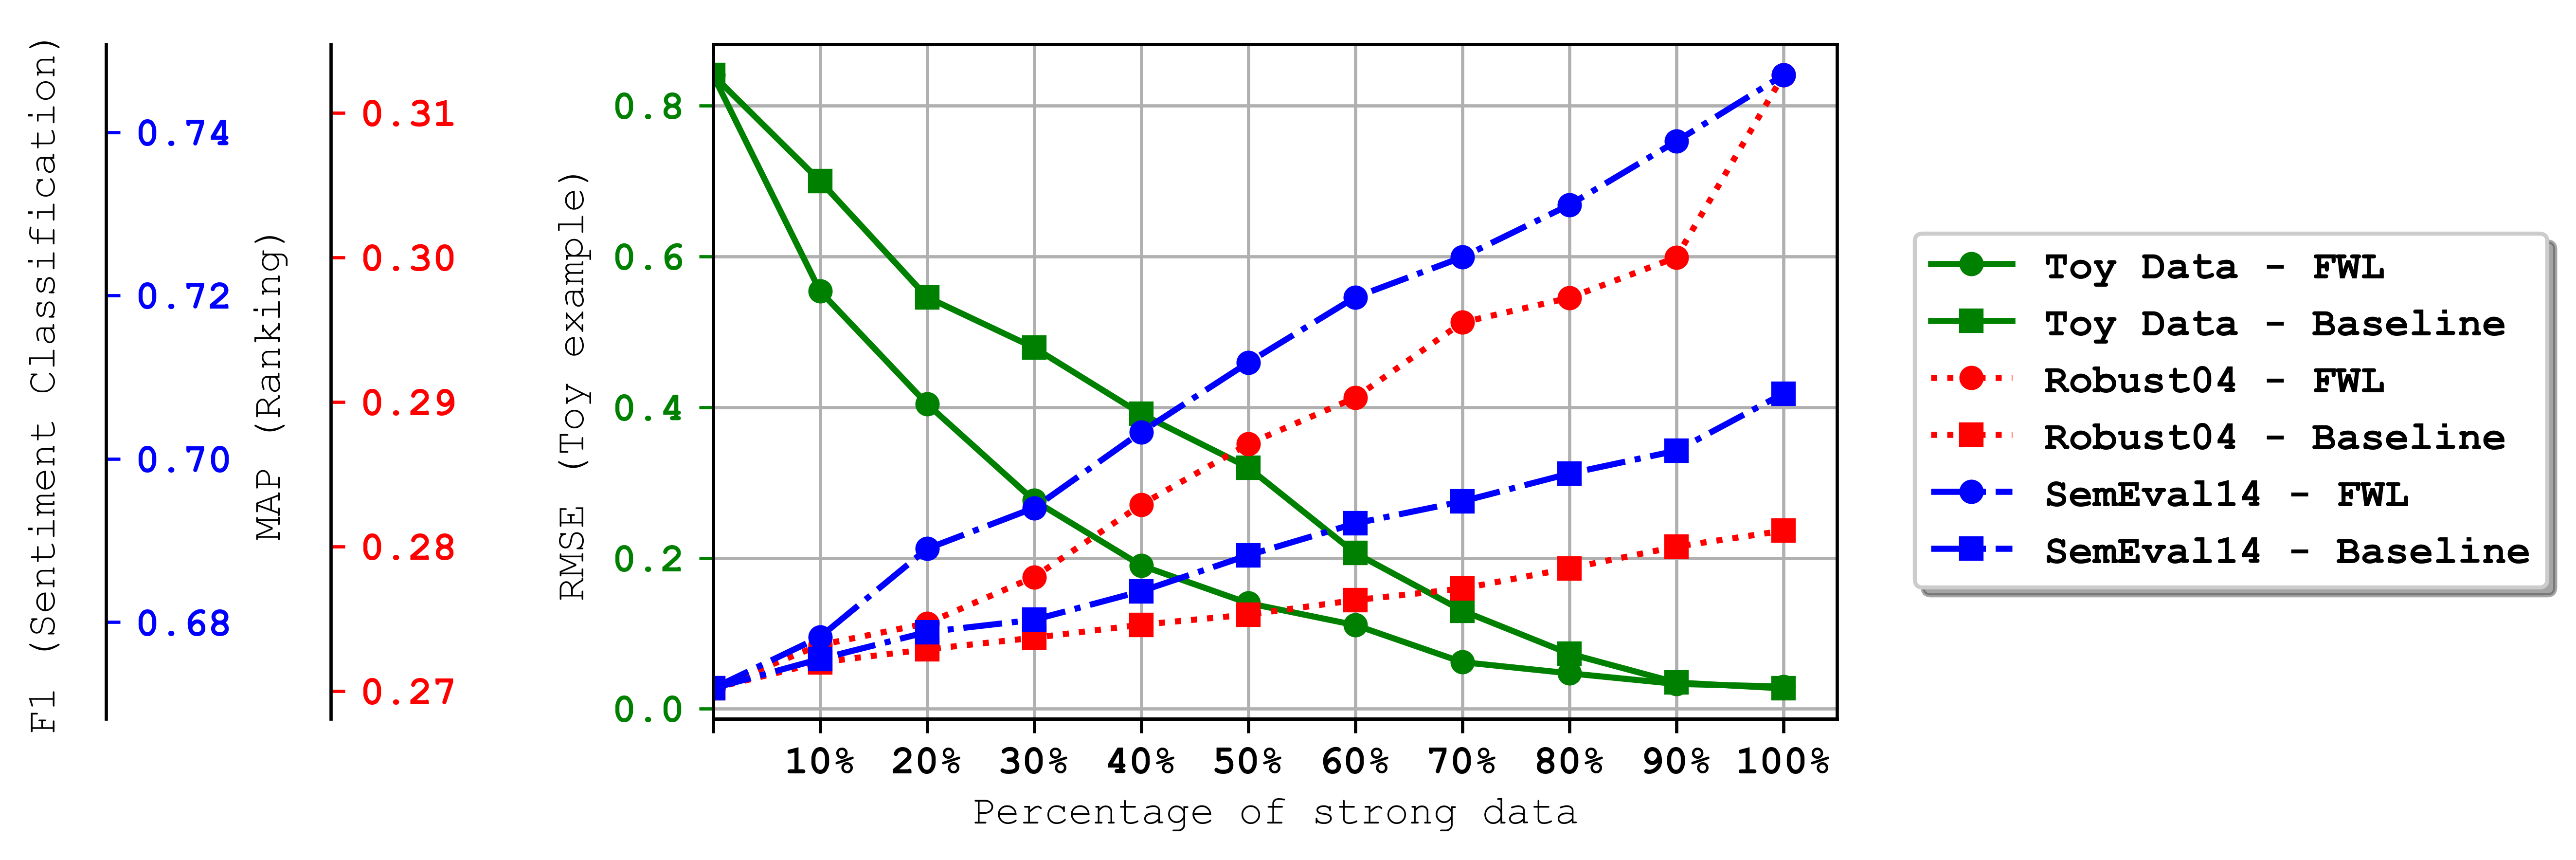
\includegraphics[width=\textwidth]{03-part-02/chapter-05/figs_and_tables/fig_data_s.png}
        \caption{\label{fig:plot_dt}\footnotesize{Models trained on different amount of strong data.}}
    \end{subfigure}%
    \caption{Performance of \fwl and the baseline model trained on different amount of data.}
    \label{fig:learning_rate}
\end{figure}
Relevant to this, we performed two types of experiments on all tasks:
%
\begin{itemize}
    \item In the first experiment, we use all the available strong data but consider different percentages of the entire weak dataset.
    \item In the second experiment, we fix the amount of weak data and provide the model with varying amounts of strong data.
\end{itemize} 
We use standard fine tuning with similar setups as for the baseline models. 
We fixed everything in the model and tried running the fine tuning step with different values for $\beta \in \{0.0, 0.1, 1.0, 2.0, 5.0\}$ in all the experiments.
For the experiments on the toy problem in Section~\ref{sec:learning_pace}, the reported numbers are averaged over 10 trials. In the first experiment (i.e., Figure~\ref{fig:plot_dw}), the size of sampled data data is: $|\mathcal{D}_s| = 50$ and $|\mathcal{D}_w| = 100$ (fixed) and for the second experiment (i.e., Figure~\ref{fig:plot_dw}): $|\mathcal{D}_w| = 100$ and $|\mathcal{D}_s| = 10$ (fixed). 

Figure~\ref{fig:learning_rate} presents the results of these experiments. In general, for all tasks and both setups, the \std learns faster when there is a \tch.
One caveat is in the case where we have a very small amount of weak data. In this case, the \std cannot learn a suitable representation in the first step, and hence the performance of \fwl is rather low, as expected. It is highly unlikely that this situation occurs in reality as obtaining weakly labeled data is much easier than strong data.

The empirical observation of Figure~\ref{fig:learning_rate} that our model learns more with less data can also be seen as evidence in support of another perspective to \fwl, i.e. \emph{learning using privileged information}~\citep{vapnik2015learning}. 


\subsection{Handling the Bias-Variance Trade-off in \fwl}
\label{sec:bias-variance}
As mentioned in Section~\ref{sec:proposed-method}, $\beta$ is a hyperparameter that controls the contribution of weak and strong data to the training procedure. In order to investigate its influence, we fixed everything in the model and ran the fine tuning step with different values of $\beta \in \{0.0, 0.1, 1.0, 2.0, 5.0\}$ in all the experiments.

%
\begin{figure}[!t]
    \centering
    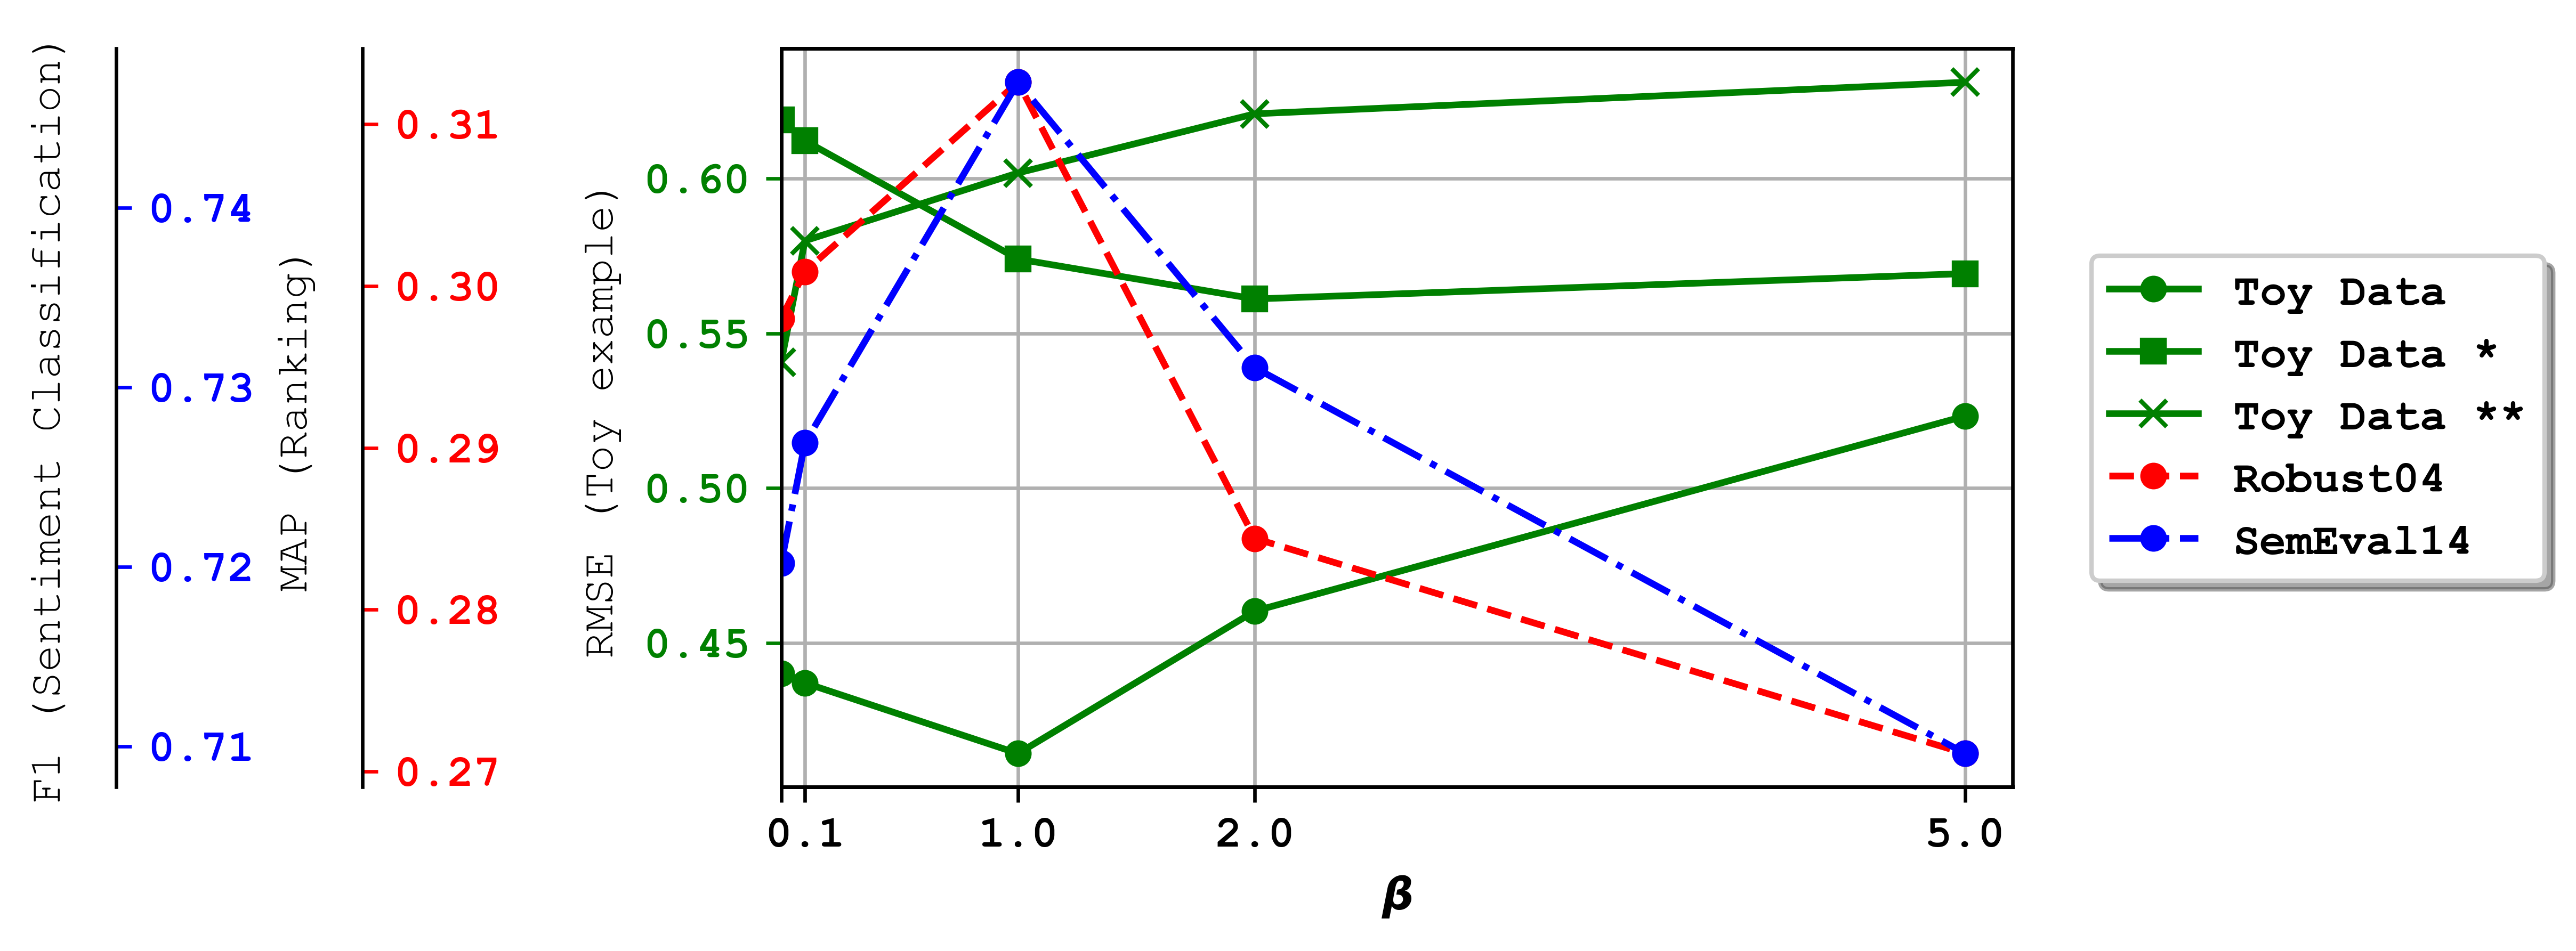
\includegraphics[width=0.8\textwidth]{03-part-02/chapter-05/figs_and_tables/plot_beta_fwl.png}
    \caption{\fontsize{8}{7}\selectfont{Effect of different values for $\beta$}.}
    \label{fig:beta}
\end{figure}
Figure~\ref{fig:beta} illustrates the performance on the ranking (on the Robust04 dataset) and sentiment classification tasks (on the SemEval14 dataset).  For both sentiment classification and ranking, $\beta=1$ gives the best results (higher scores are better).
%
We also experimented on the toy problem with different values of $\beta$ in three cases: 
1) having 10 observations from the true function (same setup as Section~\ref{sec:toy_exmpale}), marked as ``Toy Data'' in the plot, 
2) having only 5 observations from the true function, marked as ``Toy Data *'' in the plot, and 
3) having $f(x) = x + 1$ as the weak function, which is an extremely bad approximator of the true function, marked as ``Toy Data **'' in the plot.
%
For the ``Toy Data'' experiment, $\beta=1$ turned out to be optimal (here, lower scores are better). However, for ``Toy Data *,'' where we have an extremely small number of observations from the true function, setting $\beta$ to a higher value acts as a regularizer by relying more on weak signals, and eventually leads to better generalization. 
On the other hand, for ``Toy Data **,'' where the quality of the \wa is extremely low, lower values of $\beta$ put more focus on the true observations. Therefore, $\beta$ lets us control the bias-variance trade-off in these extreme cases.

We have also tested $\hat{c}_t = \eta_2(x_t) = \nicefrac{\beta}{\rm var}[\Sigma(x_t)]$.  The experiments showed that the exponential choice gives a better overall performance. 


\subsection{Sensitivity of \fwl to the Quality of the Weak Annotator}
Our proposed setup in \fwl requires defining a so-called ``\wa'' to provide a source of weak supervision for unlabelled data. In Section~\ref{sec:bias-variance} we discussed the role of the parameter $\beta$ for controlling the bias-variance trade-off by trying two weak annotators for the toy problem. 
Now, in this section, we study how the quality of the weak annotator may affect the performance of the \fwl, for the task of document ranking as a real-world problem.

\begin{figure}[t]
    \centering
    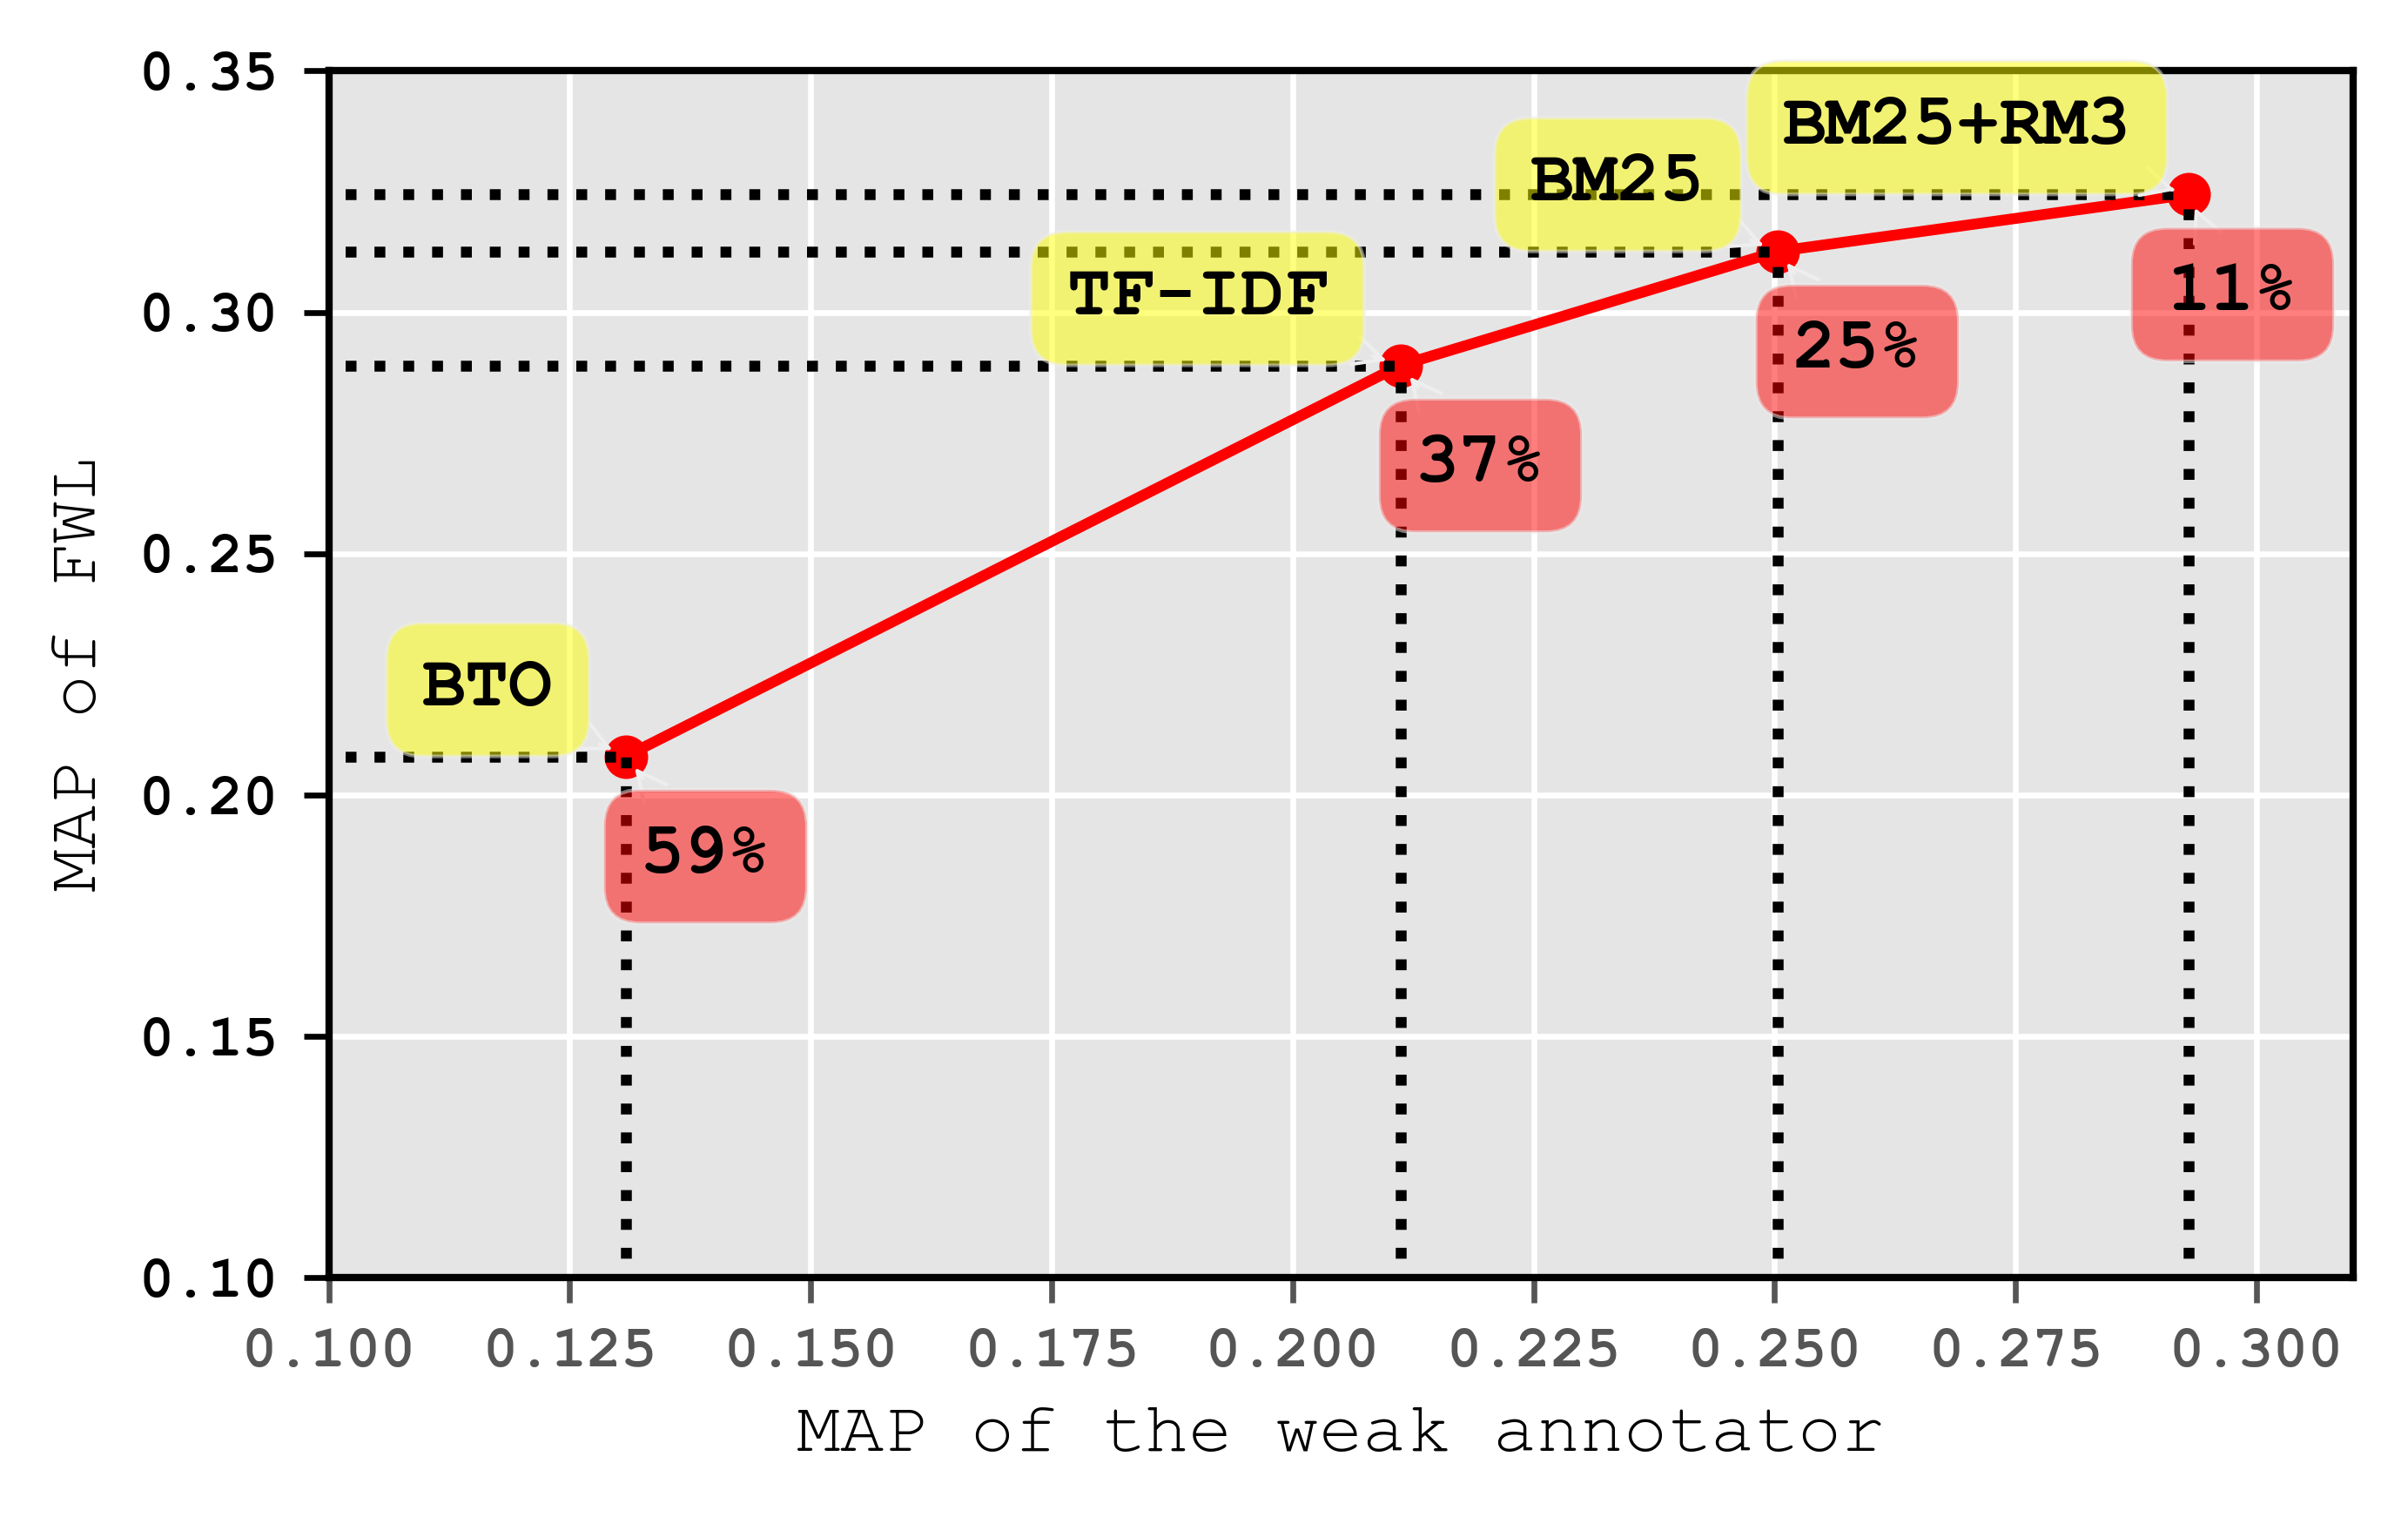
\includegraphics[width=0.7\textwidth]{03-part-02/chapter-05/figs_and_tables/plot_sensitivity_fwl.png}
    \caption{Performance of \fwl versus performance of the corresponding \wa in the document ranking task, on the Robust04 dataset.}
    \label{fig:sensitivity}
\end{figure}
To do so, besides BM25~\citep{Robertson:2009}, we use three other weak annotators: 
a vector space model~\citep{salton1973specification} with a binary term occurrence (BTO) weighting schema and a vector space model with the TF-IDF weighting schema, which are both weaker than BM25, and BM25+RM3~\citep{Abdul-jaleel:2004} that uses RM3 as the pseudo-relevance feedback method on top of BM25, leading to better labels. 

Figure~\ref{fig:sensitivity} illustrates the performance of these four \was in terms of their mean average precision (MAP) on the test data, versus the performance of \fwl given the corresponding \wa. As expected, the performance of \fwl depends on the quality of the employed \wa.
The percentage of improvement of \fwl over its corresponding \wa on the test data is also presented in Figure~\ref{fig:sensitivity}. As can be seen, the better the performance of the \wa is, the less the improvement of the \fwl would be. 


\subsection{From Modifying the Learning Rate to Weighted Sampling}
\fwl provides confidence scores based on the certainty associated with each generated label $\bar{y}_t$, given sample $x_t \in \mathcal{D}_{sw}$. We can translate the confidence score as how likely including $(x_t,\bar{y}_t)$ in the training set for the \std model improves the performance, and rather than using this score as the multiplicative factor in the learning rate, we can use it to bias the sampling procedure of mini-batches so that the frequency of training samples is proportional to the confidence score of their labels.

We design an experiment to try \fwl with this setup (\fwlnospace$_s$), in which we keep the architectures of the \std and the \tch and the procedure of the  first two steps of the \fwl fixed, but we changed the step 3 as follows:

Given the soft dataset $\mathcal{D}_{sw}$, consisting of $x_t$, its label $\bar{y}_t$ and the associated confidence score generated by the \tch, we normalize the confidence scores over all training samples and set the normalized score of each sample as its probability to be sampled. 
Afterwards, we train the \std model by mini-batches sampled from this set with respect to the probabilities associated with each sample, but without considering the original confidence scores in parameter updating.
This means that the more confident the \tch is about the generated label for each sample, the more chance that the sample has to be seen by the \std model.
\begin{figure}[t]
    \centering
    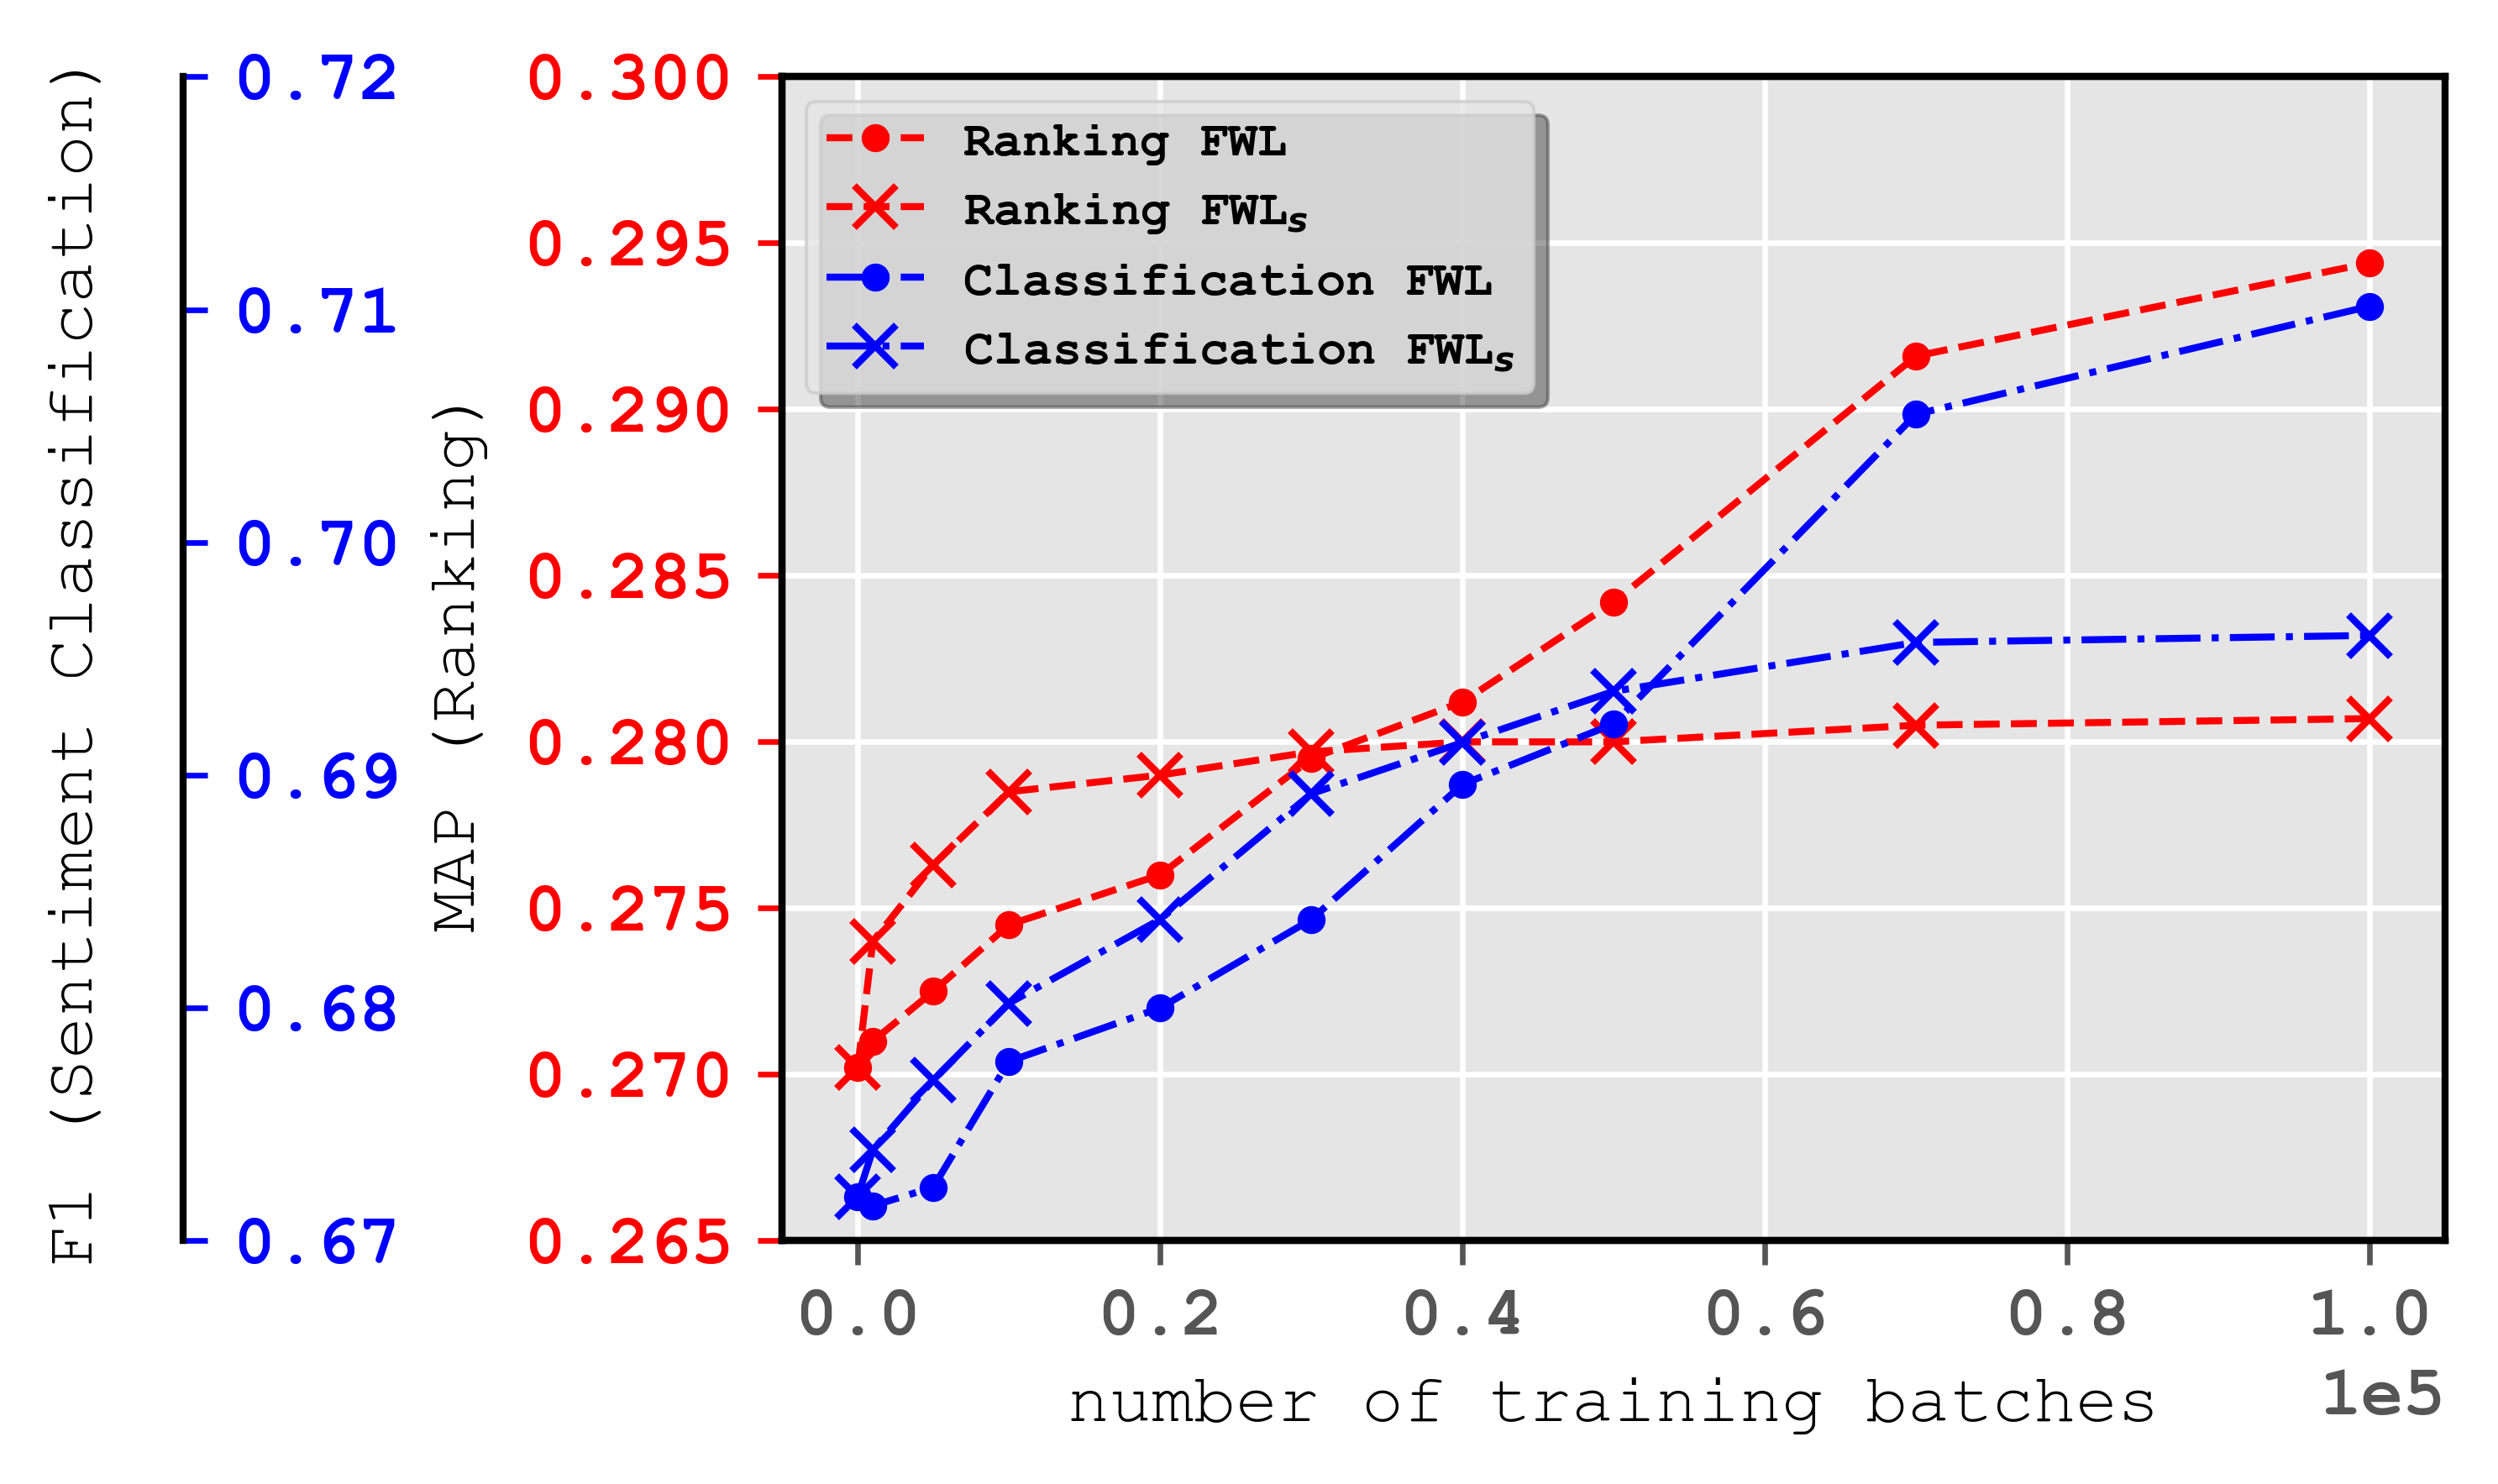
\includegraphics[width=0.7\textwidth]{03-part-02/chapter-05/figs_and_tables/plot_sampling_fwl.png}
    \caption{Performance of \fwl and \fwlnospace$_s$ with respect to different batch of data for the task of document ranking (Robust04 dataset) and sentiment classification (SemEval14 dataset).}
    \label{fig:sampling}
\end{figure}
Figure~\ref{fig:sampling} illustrates the performance of both \fwl and \fwlnospace$_s$ trained on different amounts of data sampled from $\mathcal{D}_{sw}$, in the document ranking and sentiment classification tasks. 

As can be seen, compared to \fwl, the performance of \fwlnospace$_s$ increases rapidly in the beginning but it slows down afterward. 
We have looked into the sampling procedure and noticed that the confidence scores provided by the \tch form a rather skewed distribution and there is a strong bias in \fwlnospace$_s$ toward sampling from data points that are either in or close to the points in $\mathcal{D}_{s}$, as $\mathcal{GP}$ has less uncertainty around these points and the confidence scores are high.
We observed that the performance of \fwlnospace$_s$ gets closer to the performance of \fwl after many epochs, while \fwl had already a log convergence.
%
The skewness of the confidence distribution makes \fwlnospace$_s$ to have a tendency for more exploitation than exploration, however, \fwl has more chance to explore the input space, while it controls the effect of updates on the parameters for samples based on their merit. 